%%%%% Magnetisches Feld %%%%%
%% #1 Beweis für die Existenz %%


%Some sample text to be displayed above the first subsection

%\subsection{Prinzip}

%Ein Zyklotron besteht aus Zwei hohlen, halbzylindrischen und Duanden an denen eine Spannung mit unterschiedlichem Vorzeichen anliegt, und darüber bzw. darunter liegende Magneten, die ein homogenes Magnetfeld erzeugen. Zudem gibt es einen Einlass und einen Auslass für Teilchen.

%\begin{wrapfigure}{r}{0.4\textwidth} \label{Zyklo}
%
%	\vspace{-10pt}
%	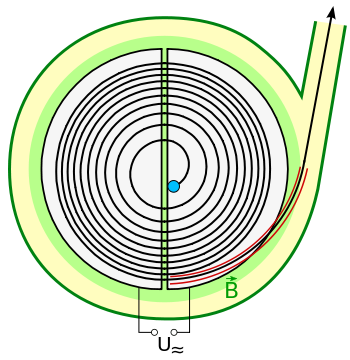
\includegraphics[width=0.35\textwidth]{Zyklotron_Prinzipskizze02.png}
%	\vspace{-13pt}
%	\caption{Prinzipskizze eines Zyklotrons}
%	\vspace{-5pt}	
%	
%\end{wrapfigure}

%\subsubsection{Anwendung}

% Some Formula:

%\begin{equation}
%	x= \frac{y \cdot 13 \pi z}
%			{\cos \alpha}
%\end{equation}

%%%%%%%%%%%%%%%%%%%%%%%
% Eigentlicher Beginn %
%%%%%%%%%%%%%%%%%%%%%%%


Man hat festgestellt, dass es noch ein weiteres Etwas mit Feldeigenschaften gibt, das Ähnlichkeiten mit dem Gravitationsfeld zeigt. Die wichtigste gemeinsame Eigenschaft ist, dass Kräfte auf bestimmte Körper ausgewirkt werden können, ohne dass ein erkennbares Medium gibt: Der magnetische Effekt ist auch im Vakuum zu beobachten. 

Diese Effekt kann durch eine Mehrzahl Ereignisse ausgelöst werden. Siehe dazu \referenz{sec:UrsachenEigenschaften}.




